\section{introduction}
\label{sec:introduction}
Are persuasive text messages more effective when expressed in comic form? Text messages abound, asking us to act, either towards personal wellness goals (e.g. in an exercise app:``you need 2,000 more steps to reach 10,000 steps for the day''), reminders (e.g. push notifications from a task tracking app: ``pick up prescription from the pharmacy at 6PM''), or appeals from charities online (e.g. from a Wikipedia campaign on the Wikipedia homepage: ``If everyone reading this donated \$5 our fundraiser would end today. Please donate to keep Wikipedia free.''). Making these short text messages more effective has important implications in stimulating behavior, especially for non-profits and governmental agencies interested in alleviating public goods dilemmas.

There is a rich history of prior work in psychology that has examined how variations in the construction of the text message alter decisions. In a seminal paper,~\textcite{tversky1981framing} examined information framing: can we elicit different decisions, by describing the outcome either as a loss or a gain, even though the two messages are indistinguishable in terms of expected utility? They found that individuals are risk-seeking when confronted with certain loss and risk-averse in the presence of gains. Cialdini examined the introduction of social proofs in two different contexts: towel re-use in hotels~\parencite{goldstein2008room}, reduction of power consumption~\parencite{schultz2007constructive}. In the former study, replacing the standard text message in hotels asking the customer to re-use towels with the social proof (e.g. ``75\% of the people in this hotel have re-used their towels'') increased towel re-use. The latter study had an intriguing result---while introducing the social proof in the message \textit{did not} reduce overall energy consumption, adding emoticons to the message with the social proof made a difference. Specifically, they added a smiley face `\smiley{}' when the customer consumed less energy than average, and a frowny face `\frownie{}' when their energy consumption was worse than average. By adding emoticons average energy consumption decreased. The~\textcite{schultz2007constructive} study motivates us to examine the role of the comic form, a highly expressive and affective medium, in communicating messages intended to stimulate a specific behavior.

\textcite{scott1993understanding} defines comics as ``juxtaposed pictorial and other images in deliberate sequence, intended to convey information and/or to produce an aesthetic response in the viewer.''  The simple and humorous nature of a comic makes it a unique medium for delivering informative and memorable messages; the use of metaphor in comics can make the underlying meaning vivid and more memorable than using a straightforward description~\parencite{McDermottPB18,scott1993understanding}. There has been significant prior work in educational contexts: illustrating scientific facts~\parencite{McDermottPB18}, educating end-users about computer-security \footnote{Also used in introducing software: see~\url{https://www.google.com/googlebooks/chrome/big_00.html} for an example.}~\parencite{Zhang-Kennedy:2017:SCI:3206217.3206282}, communicating with multi-lingual audiences~\parencite{cary2004going, miguel2005ethnic}. 

\begin{wrapfigure}{R}{0.23\textwidth}
    \centering
    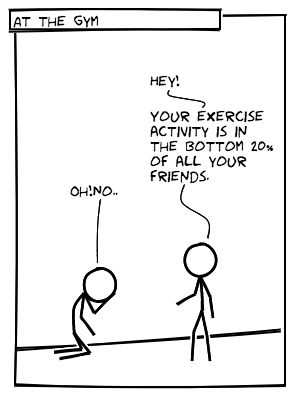
\includegraphics[width=0.21\textwidth]{figures/intro_new.png}
  \vspace{-10pt}
  \caption{An example single comic panel in abstract comic form.} \label{fig:intro}
  \vspace{-10pt}
\end{wrapfigure}

Despite the importance of the comic form in contemporary culture, and the use of the comic form in educational settings, there is surprisingly limited work examining the effects of the comic form to stimulate behavior. In particular, we focus on the use of an abstract comic form. By an abstract representation, (see~\Cref{fig:intro} for an example) we mean that the comic de-emphasizes character detail (face, eyes, etc.) or details about the locale. As~\textcite{scott1993understanding} points out, using abstract representations for the comic allows the reader to project themselves onto the comic character. The abstract form has an additional benefit: since the form is visually spare, it allows for comic panel algorithmic synthesis and for the personalization of messages. In this paper, we used a three-panel comic in abstract form.

We use an online charitable donation task for our experiment: the task is a  single-shot task, contributes to the public good with distant, non-exclusive rewards, occurs frequently, and easily tested for at scale. We chose a charity associated with Autism (Organization for Autism Research) for our experiment.

Thus, in this work we answer two research questions in the context of the online charitable donation task:
\begin{description}
    \item[RQ1:] Does the use of the abstract comic form increase the level of donation over the plain text message? \footnote{The abstract comic includes the same text from the plain text condition. Thus both conditions indicate the same expected utility.}
    \item[RQ2:] What is the effect of introducing a social proof in the abstract comic, when compared to the comic without the social proof?
\end{description}

We would like to emphasize that it is unclear at the outset if a message in comic form ought to make any difference towards a charitable donation. An argument in favor is that comics communicate affect well and are an important element of our visual culture; an argument against is that from rational actor theory in classical Economics, since the comic includes the text message used in the text-only condition and thus cannot alter the expected utility, the comic ought to serve as an irrelevant factor. To the best of our knowledge, this is the first study to examine the persuasive power of an abstract comic in an online public good setting with distant and non-exclusive rewards. 

We ran the experiment using Amazon Mechanical Turk ($n=307$; we paid each participant above minimum wage, at \$10.0/hr) where we randomly assigned each participant to one of the three conditions ('a plain text message', 'abstract comic', 'abstract comic with social proof'). The two comic conditions include the text used in the plain text condition. The social proof case adds one additional phrase to the comic that reveals the norm.

We performed a careful Bayesian analysis to analyze the data. We agree with the observations by~\textcite{Kay2016}, that beyond the impact on experimental replicability, shifting the question from ``did it have an effect?'' to ``how strong was the effect?'' is important to the HCI community. Two additional ideas---transparency, impact small-$n$ studies---motivate our use of Bayesian analysis. First, with a Bayesian model, the researcher foregrounds all the aspects of the model; there are no modeling assumptions that need checking, not already foregrounded in the model description. Thus the model and the results are amenable to further scrutiny. Second, a Bayesian model is valid at \textit{every} value of $n$ (the number of observations); we do not have to wait for $n\geq 30$ to satisfy assumptions of Normality. For small $n$ values, the result is of course affected by the choice of the prior; but by using weakly informative priors, we can ensure that the prior doesn't dominate inference. In a sense, as ~\textcite[][Chapter 9]{McElreath2015} mentioned, Bayesian models make the \textit{most conservative} inference given the data.


\textbf{Our findings:} We show that using the comic has a significant increase in donations over the plain text conditions, with a medium to large effect size of $0.59$. Thus we can answer \textbf{RQ1} affirmatively. To answer \textbf{RQ2}, we show that while the comic with social proof increases the donation level over the comic without the norm, the effect size is very small ($0.11$) and the increase is not significant. To summarize, the comic form significantly increases donations over the plain text, but the presence of the social proof is not effective. We caution that the result holds for single-shot, public goods tasks. To fully understand the value of incorporating the social proof in the comic, for specific longitudinal tasks such as dieting, with distant, exclusive rewards and where habits can confound, we need future research.  

\textbf{Design Implications:} The primary design implication of our findings: helping non-profits and governmental agencies with their online messaging strategies as they work to alleviate public goods dilemmas. In particular, public-goods dilemmas that require single-shot decisions (online charitable donations) are opportune candidates for intervention. We believe that these agencies can easily include the use of the comic form as part of their overall messaging strategy because the simplicity of the abstract comic form allows it to be easily synthesized (as we discuss in~\Cref{sub:framework}, towards of the end of this paper) and to additionally incorporate social proofs. 


The rest of this paper is organized as follows. In the next section, we discuss related work.~\Cref{sec:relatedwork} introduces two motivating ideas: the abstract comic form, and the idea of the social proof.~\Cref{sec:Method} introduces our experimental method and in~\Cref{sec:Study on Behavior Results} we present our Bayesian analysis. In~\Cref{sec:Model Criticism}, we analyze the model for convergence and also discuss alternative models.~\Cref{sec:Discussion} summarizes the main findings, discusses how we could algorithmically synthesize the comic panels and then identifies limitations. We present our conclusions in~\Cref{sec:Conclusion}. 
